\section{Lab 1 - Introduction to FPGA's and VHDL}

\subsection{Introduction}
This lab will introduce you to the Altera DE2-115 FPGA Development Board. The DE2-115 contains all of the hardware necessary to prototype and create various hardware configurations on the Altera Cyclone IV FPGA chip that will be used throughout the course of this lab. By completing this lab, you will have an understanding of all the hardware contained on the FPGA development board, along with an understanding of how to connect peripherals to the development board. Lastly, this lab will go over the standard template for designing hardware in the VHDL programming language. All this will be accomplished by following the Quartus II introductory packet along with the following activities.

\subsection{The DE2-115 FPGA Development Board}

\begin{figure}[H]
	\centering
	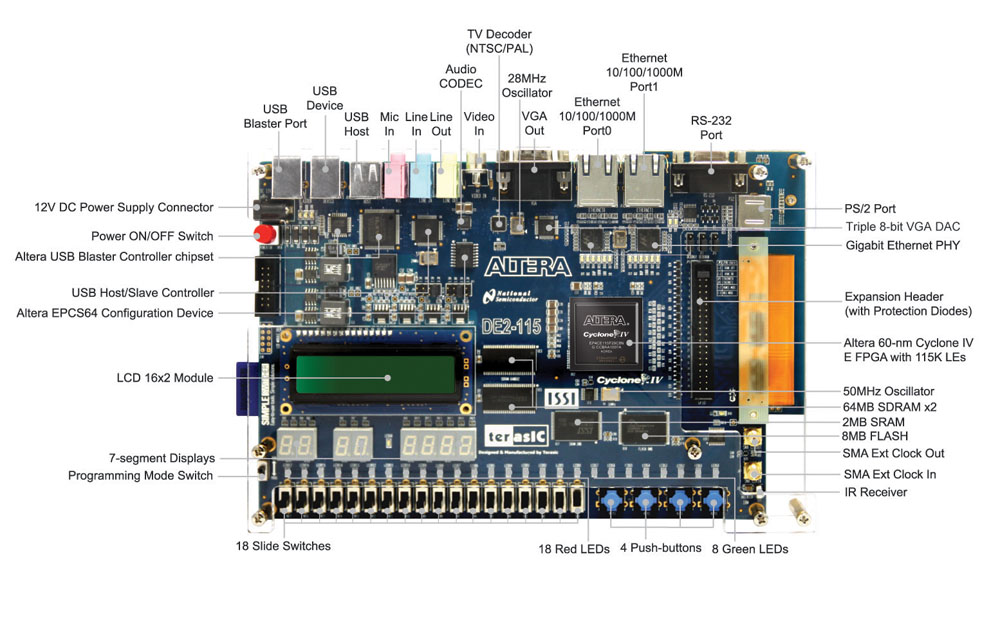
\includegraphics[width=170mm]{Lab1/figures/DE2-115.jpg}
	\caption{The DE2-115 FPGA Development Board}
	\label{fig:DE2-115}
\end{figure}

\begin{figure}[H]
	\centering
	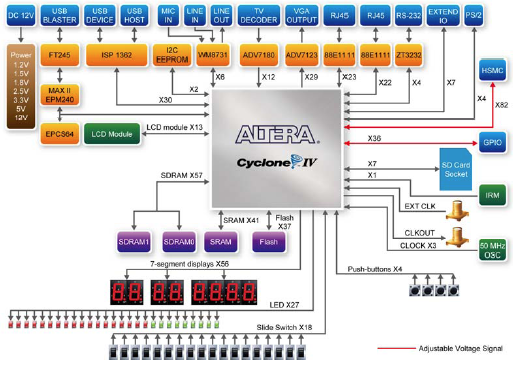
\includegraphics[width=170mm]{Lab1/figures/DE2-115Block.png}
	\caption{The DE2-115 Block Diagram}
	\label{fig:DE2Block}
\end{figure}

\subsection{Pre-Lab}

Before attempting this lab, you should complete the following:

\begin{itemize}
	\item Download and install the \emph{Quartus II 13.0 Web Edition Software} from the Altera website to your personal computer
	\item Download and install the \emph{Altera University Installer Software} located at http://www.altera.com/education/univ/software/upds/unv-upds.html
	\item Download and read the following documents from the Sakai Resources pags;  \emph{DE2-115 User Manual}, \emph{Quartus II Introduction}
\end{itemize}
 
\subsection{Working with Quartus II}

\subsubsection{Creating a New Project}
\begin{enumerate}
	\item In order to begin working on your first FPGA project, you must open the program Altera Quartus II. To begin a new project goto  {\bf File $\rightarrow$ New Project Wizard} as shown in figure \ref{fig:step1}

	\begin{figure}[H]
		\centering
		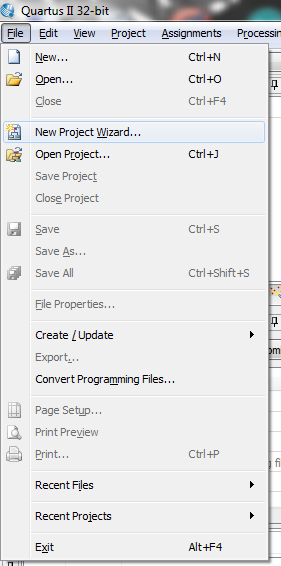
\includegraphics[width=45mm]{Lab1/figures/step1.png}
		\caption{Create a new project menu}
		\label{fig:step1}
	\end{figure}

	\item When the \emph{New Project Wizard} window opens click {\bf NEXT}

	\item Create a folder in your Z-drive called \emph{FPGA Lab}

	\item Create a folder in FPGA Lab called \emph{lab1}

	\item Set the working directory to lab1

	\item Name the project \emph{lab1}

	\item Click {\bf NEXT} to proceed

	\item Skip this step, click  {\bf NEXT} to proceed

	\item Under Device Family select \emph{Cyclone IV E}, set the package to \emph{FBGA}, pin count to \emph{780}, and speed grade to \emph{7}. In the Available devices list, look for and select \emph{EP4CE115F29C7} as shown in figure \ref{fig:step2}.
	

	\begin{figure}[H]
		\centering
		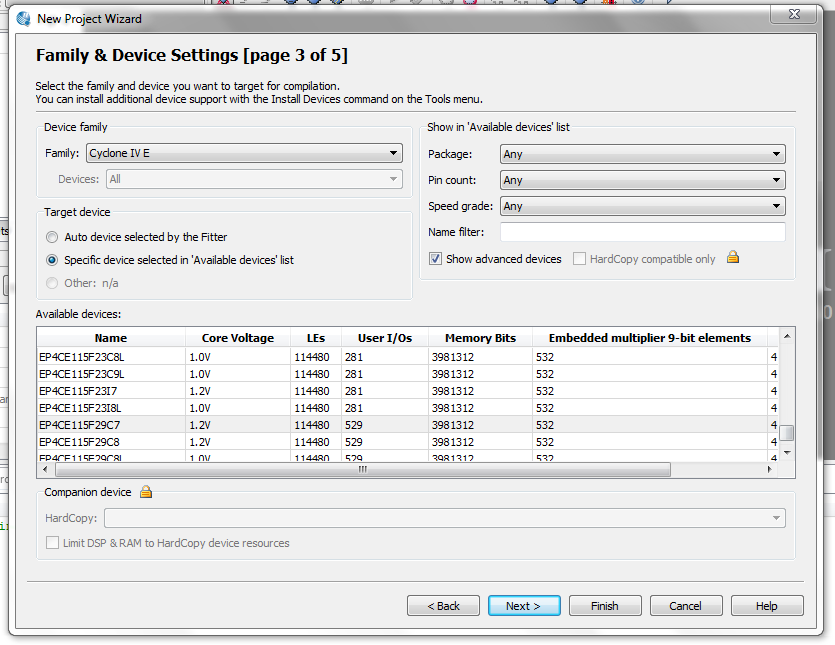
\includegraphics[width=100mm]{Lab1/figures/step2.png}
		\caption{Device selection menu}
		\label{fig:step2}
	\end{figure}

	\item Click {\bf FINISH} to begin your new project

\end{enumerate}

\subsubsection{Creating an Empty File}
\begin{enumerate}

	\item Goto {\bf File $\rightarrow$ New $\rightarrow$ VHDL File $\rightarrow$ OK } as shown in figure \ref{fig:newfile}

	\begin{figure}[H]
		\centering
		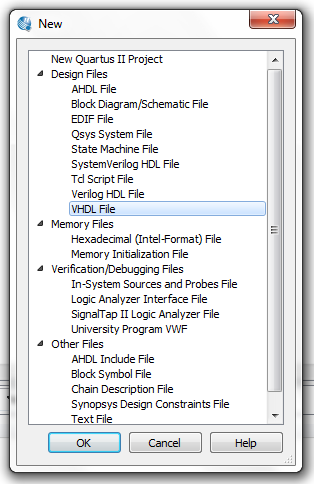
\includegraphics[width=50mm]{Lab1/figures/newfile.png}
		\caption{Create a new file menu}
		\label{fig:newfile}
	\end{figure}

	\item Save this new file by going to {\bf File $\rightarrow$ Save As $\rightarrow$ \emph{lab1.vhd} $\rightarrow$ SAVE} as shown in figure \ref{fig:saveas}

	\begin{figure}[H]
		\centering
		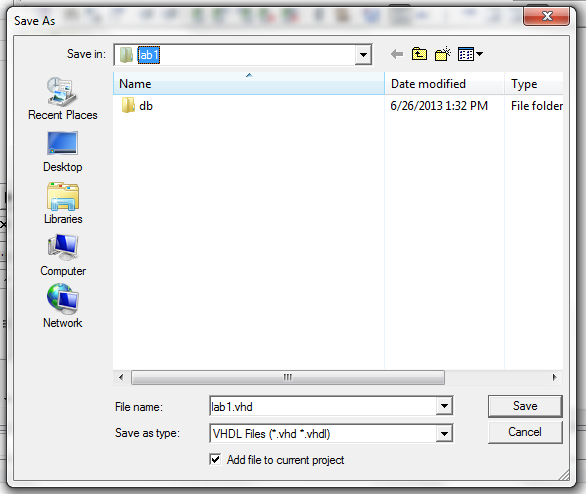
\includegraphics[width=65mm]{Lab1/figures/saveas.png}
		\caption{Save As dialog box}
		\label{fig:saveas}
	\end{figure}

\end{enumerate}

\subsubsection{Writing VHDL Code}

The following code block shows how to interact with the switches and LEDs on the DE2-115. Notice how the program begins with importing the ieee library which contains all of the basic logic primitives as established within the IEEE standard 1164. When working in industry it is common for large companies to create their own libraries as well. Every VHDL file should contain at least one entity (module) that is the same as the name of the file. An entity contains information about the structure of the module such as how many inputs/outputs (I/O) and what type of logic to expect at the I/O. Finally we define the entity in an architecture block, this section does the work on the hardware. As can be seen, this code is setting the red LEDs as defined in the array to the accompanying switches on the board. Take note on the use of comments throughout the code, comments begin with two dashes (--) and should always be used to describe what you are trying to accomplish, this way someone else who reads your code will understand it easily and your code will look more professional. 

\begin{lstlisting}
-- Import logic primitives
LIBRARY ieee;
USE ieee.std_logic_1164.all;

-- Simple module that connects the SW switches to the LEDR lights
ENTITY lab1 IS
PORT ( SW: IN STD_LOGIC_VECTOR(17 DOWNTO 0); -- Initialize switches as an input
	LEDR: OUT STD_LOGIC_VECTOR(17 DOWNTO 0)); -- Initialize red LEDs as an output
END lab1;

-- Define characteristics of the entity lab1
ARCHITECTURE Behavior OF lab1 IS
BEGIN
	LEDR <= SW; -- Assign each switch to one red LED
END Behavior;
\end{lstlisting}

\subsubsection{Setting Pin Assignments}
The Cyclone IV chip on the DE2-115 contains 780 pins. The majoprity of these pins have copper traces to the hardware the control on the development board. As a result, Altera has provided a file that contains all of the pin assignments so that you can interface directly with the pins in your VHDL code. To set the pin assignments:

 \begin{enumerate}  
 
	\item Goto {\bf Assignments $\rightarrow$  Import Assignments $\rightarrow$  Select \emph DE2-115.qsf} as shown in figure \ref{fig:importassign}.This file can be dowloaded from the Altera website
	
	\item Then click {\bf ADVANCED $\rightarrow$ check Global Assignments $\rightarrow$ Ok} as shown in figure \ref{fig:advancedimport}

\end{enumerate}

\begin{figure}[H]
	\centering
	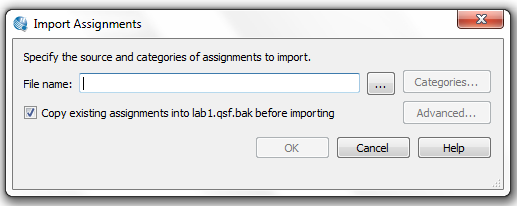
\includegraphics[width=70mm]{Lab1/figures/importassign.png}
	\caption{Import assignments dialog box}
	\label{fig:importassign}
\end{figure}

\begin{figure}[H]
	\centering
	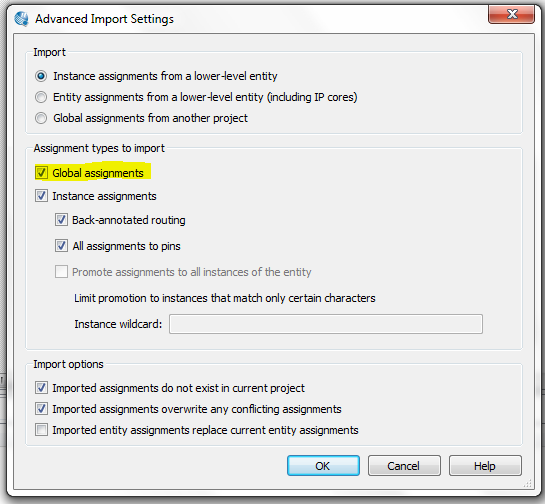
\includegraphics[width=85mm]{Lab1/figures/advancedimport.png}
	\caption{Import assignments advanced options menu}
	\label{fig:advancedimport}
\end{figure}

\subsubsection{Compiling Hardware}

\begin{enumerate}

	\item To begin compiling your hardware, {\bf Processing $\rightarrow$ Start Compilation} or you may press \emph{Ctrl + L} on your keyboard

\end{enumerate}

If the project compiles successfully, you may proceed to uploading the hardware. Otherwise if you have any errors you should debug your code. It is helpful to note that the first error should be solved first which will make it easier to solve the other errors. A succefull compilation will look like figure \ref{fig:compileresuts}.

\begin{figure}[H]
	\centering
	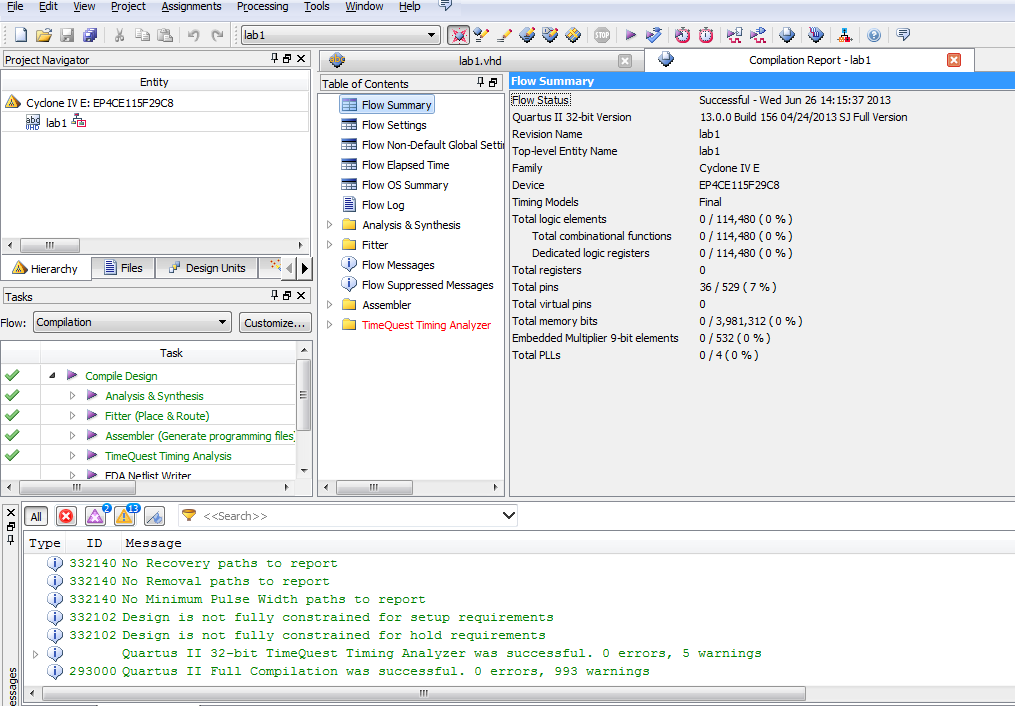
\includegraphics[width=100mm]{Lab1/figures/compileresults.png}
	\caption{Successful completion of compilation}
	\label{fig:compileresuts}
\end{figure}

\subsubsection{Testing Hardware with Waveforms}

All hardware implementations should be tested for correctness before uploading to the FPGA device. To accomplish this, please follow the tutorial titled \emph{Quartus\_II\_Simulation.pdf} listed under Sakai resources.

\subsubsection{Uploading Hardware to Device}

Once the hardware has compiled successfully, goto {\bf Tools $\rightarrow$ Programmer} to open the hardware upload options. There are two typical modes for uploading hardware and it is important to understand when to use them. This can be seen in figure \ref{fig:uploadmethod}.


\begin{figure}[H]
	\centering
	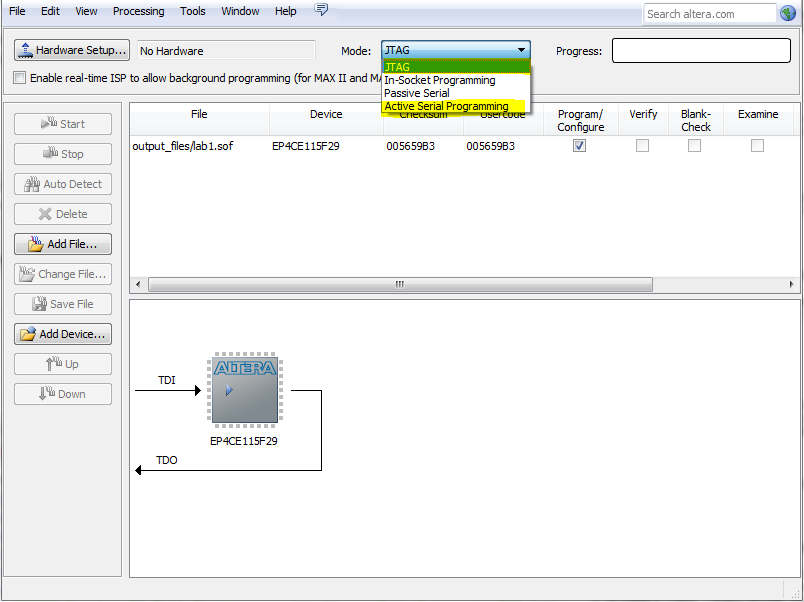
\includegraphics[width=100mm]{Lab1/figures/uploadmethod.png}
	\caption{Modes for uploading hardware to the FPGA device}
	\label{fig:uploadmethod}
\end{figure}

\begin{enumerate}

	\item JTAG or Joint Test Action Group

	\begin{itemize}
	
		\item This method loads the hardware directly to the FPGA chip
		
		\item The FPGA is unable to save its current state so if the power is turned off the programmed hardware will disappear
		
		\item To program the FPGA with this method all you need to do is connect the USB cable to the development board and ensure that under {\bf Hardware Setup} that USB-Blaster is selected. Then you must goto {\bf Add Files} and add your compiled \emph{lab1.sof} file
		
		\item Press {\bf START} to upload your hardware, in a few moments you should see your development board behaving as instructed by your code
		
	\end{itemize}

\item Active Serial

	\begin{itemize}
		\item This method loads the hardware on to the on-board configuration device. What this means is that the hardware description is saved into memory and is loaded onto the FPGA chip whenever the board is powered on. This method is more desirable because it allows the FPGA to work without being connected to the computer and only to an external power source.
		
		\item Before beginning this method you should first check that under {\bf Assignments $\rightarrow$ Device $\rightarrow$ Device and Pin Options} are configured in the same way as figure \ref{fig:activeserialconfig}, if not you must set the configuration scheme to \emph{Active Serial} and also set  the configuration device to \emph{EPCS64}. If this was not set you must recompile your hardware.

		\begin{figure}[H]
			\centering
			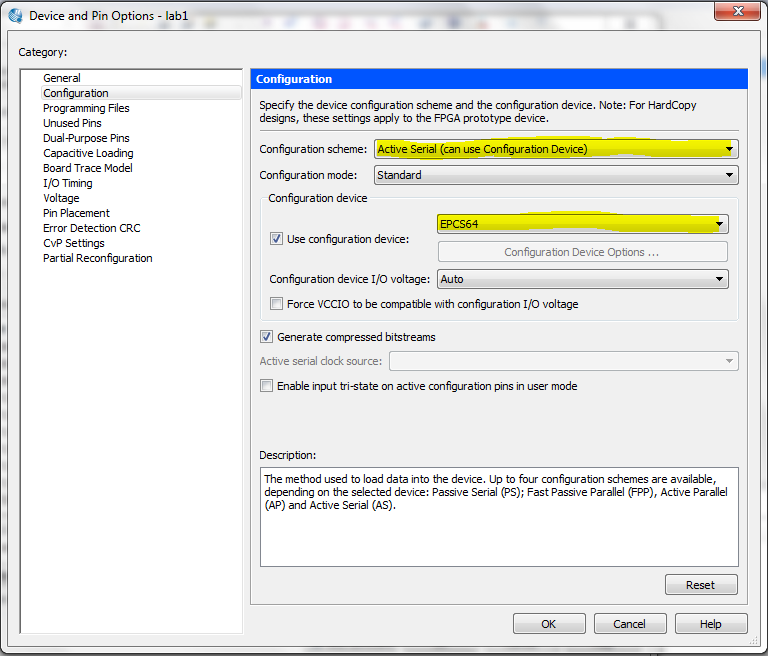
\includegraphics[width=100mm]{Lab1/figures/activeserialconfig.png}
			\caption{Active Serial Configuration Settings}	
			\label{fig:activeserialconfig}
		\end{figure}

		\item Next once again ensure that the hardware is set to \emph{USB-Blaster} and that the mode is set to \emph{Active Serial}
		
		\item Click on {\bf Add Files}, and select \emph{lab1.pof}
		
		\item Ensure that the development board is switched to \emph{PROG}
		
		\item Click {\bf START} to begin programming. This method takes slightly longer
		
		\item Switch the board back into the \emph{RUN} position and verify that your logic is behaving properly
		
	\end{itemize}

\end{enumerate}

\subsection{Activities}

\subsubsection{Implementing Logic}

Implement the hardware from the circuit in Figure \ref{fig:circuit1}. The inputs should come from SW(1) and SW(2) and the output should be shown on any of the available LEDs. Use the implemented circuit to test and create a truth table with your results and place it within a comment in the program file.

\begin{figure}[H]
	\centering
	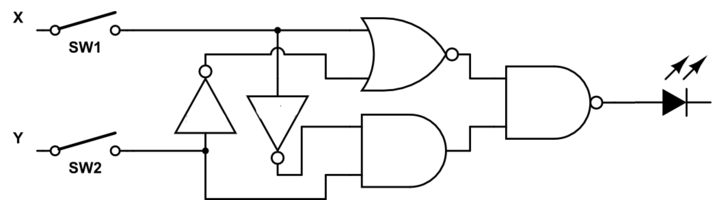
\includegraphics[width=100mm]{Lab1/figures/circuit1.png}
	\caption{Circuit for activity 1}
	\label{fig:circuit1}
\end{figure}

\subsubsection{7 Segment Display Decoder}

The 7-segment display is comprised of 7 LEDs that are arranged in such a way that allows for the creation of the numbers 0-9 and a select few characters with some clever use. Figure \ref{fig:7seg} shows the block diagram and output table. Your task is to create a 4 input, 7 output decoder that will display a number from 0-9 and the letters A-F. To accomplish this task, you should program the switches SW(0) - SW(3) to act as a 4-bit input to the decoder and output the result across all of the displays, HEX0 - HEX7.

\begin{figure}[H]
	\centering
	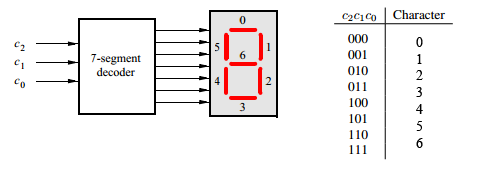
\includegraphics[width=100mm]{Lab1/figures/7seg.png}
	\caption{7 segment display and decoder}
	\label{fig:7seg}
\end{figure}

{\bf Tips:} 
\begin{itemize}
	\item You should create two entities, one labled part2 that contains the logic for the switch input and output to the displays and another labled bcd7seg that acts as a decoder for the display.
	
	\item The eight 7 segment displays can be accessed with the 7-bit signal vectors HEX0\ldots HEX7. For example, to output to the first display (HEX0) you can either set each bit individually (HEX0(5) <= `0';) or set the whole vector with (HEX0 <= `00000000') which would display the number 8. Keep in mind that the LED segments use inverted logic.
	  
	\item Figure \ref{fig:7segreference} shows how to correctly display all the required characters.
\end{itemize}

\begin{figure}[H]
	\centering
	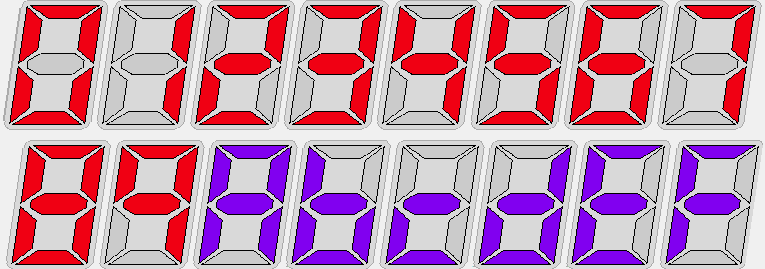
\includegraphics[width=100mm]{Lab1/figures/7segreference.png}
	\caption{7 segment displays showing all combinations for 0-9 and A-F}
	\label{fig:7segreference}
\end{figure}

\subsection{Lab Report}

Your lab report should be upload to Sakai in a zip folder that includes; your commented VHDL code, your VHDL test bench, a pdf of your waveforms, and a text file answering any questions from the activities.


